\graphicspath{{fig/sheep/}}

\chapter{Case study I: flocking sheep}
\label{cha:sheep}

In \cref{cha:sim_studies} we showed that it is possible to infer the parameters
of a number of agent-based models from simulated data. Performing simulation
studies before attempting inference on real data is advisable as it allows an
opportunity to troubleshoot and assess the accuracy of our inference schemes.
The schemes constructed to perform inference on simulated data can now be
reused with little-to-no-alteration to perform inference on real data. With the
confidence instilled by the success of our simulation studies, if we find our
schemes unable to fit a model to \emph{real} data, we can be confident that
this is because of a discrepancy between the model and data, rather than an
error in our fitting process or our implementation of it.

This chapter shall focus on data of flocking sheep, unseen before in the
literature. Aerial footage of flocking sheep was recorded by a commercially
available drone. The position of each individual sheep was extracted from the
captured video footage using custom tracking software. In total, three flocking
sequences were extracted and analysed. The flocking events were captured and
their data extracted by Hayley Moore (thesis in preparation). Global models
considered in \cref{sec:global_models} will be fit to these sequences. The
resulting fits will be assessed for validity and ranked for performance by
Akaike Information Criteria.

\section{Flocking data}
\label{sec:data}

Aerial footage of flocking sheep was captured with a commercially available DJI
Phantom $3$ drone equipped with a built in high-definition camera, representing
a frame resolution of $4000\times3000$ pixels. This video footage was recorded
at a rate of $24$ frames per second. In total, three distinct flocking events
were captured and analysed. Each flocking event involved the same flock of $45$
sheep.

The recorded flocking events took place in large open fields: a natural
environment with which the sheep were already familiar. Flocks were recorded in
familiar terrain in an attempt to observe the most natural flocking events, and
to minimise the effect which an unfamiliar environment may have on the flock
dynamics. In some cases the flocking events were initiated by the movements of
a quad bike, but were then left to develop naturally and unprompted. Events
generally took place away from hard boundaries, such as fences and trees, but
the influence of these objects from a distance cannot be ruled-out.

Custom tracking software was constructed to determine the position of each
sheep in every video frame. To correct for the movement of the drone due to
external influences, such as wind, the resulting frames were transformed with
respect to `reference' points. Reference points are stationary and identifiable
features present in all of the captured frames. Example reference points
include field boundaries, fence posts and trees.

Having corrected for extraneous drone-movement, the captured frames were then
thresholded to separate the pixels representing sheep from their surrounding
environment. Kalman filtering and the Hungarian algorithm were then used to
track the positions of individual sheep between frames. Having linked the
positions of sheep between frames, the trajectories of motion of every
individual could be reconstructed. \cref{fig:sheep_frame} shows the positions
of sheep in a single video frame, overlain are the positions of these sheep in
previous frames.

\begin{figure}[tbp]
  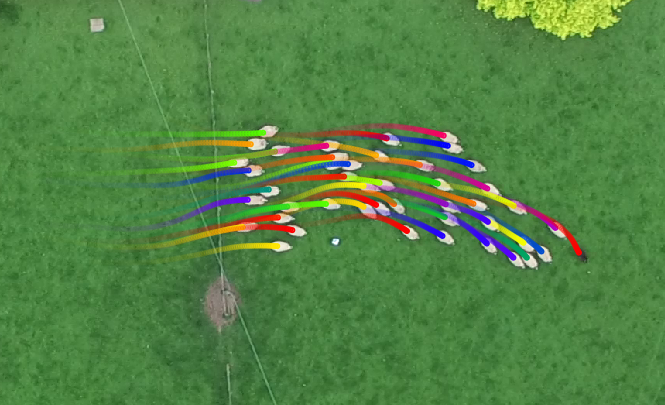
\includegraphics[width=0.8\textwidth]{traj0130_crop.png}
  \caption{A visualisation of data realised from a single flocking event. The
    faint vertical line seen passing through the image shows a boundary fence
    which was located here previously. The position of each sheep in every
    video frame was extracted using custom tracking software. Coloured lines
    represent the positions of sheep in previous frames. Each flocking event
    tracked the movements of $45$ sheep over $\approx200$ frames. A single
    flocking sequence then represents approximately $45\times200=9,000$
    observations. Footage was recorded at a rate of 24 frames per second, and so
    each sequence represents $\approx10$\,seconds of raw footage.}
  \label{fig:sheep_frame}
\end{figure}

Having realised the trajectories of each individual it is then a simple process
to determine the velocity, speed and direction of motion of each individual.
Using \cref{eq:alignment} it is possible to compute the mean polarisation of
the flocks in each sequence. The attributes of each flocking event are
summarised in \cref{tab:data_summary}. We see that sequences are broadly
similar: representing highly-polarised flocks moving at similar speeds.

\begin{table}[tbp]
\begin{tabular}{@{}crrrr@{}}
\toprule
Sequence & Frames & Sheep & Mean speed (px\,s$^{-1}$) & Mean alignment \\
\midrule
1 &    192 &     45 &      4.20 &          0.99 \\
2 &    183 &     45 &      3.26 &          0.98 \\
3 &    194 &     45 &      4.25 &          0.97 \\
\bottomrule
\end{tabular}
\caption{Summaries of the three flocking sequences analysed in this chapter.
  Each sequence involved a flock of the same $45$ sheep, recorded over
  $\approx200$ frames. As the data was recorded at a rate of $24$ frames per
  second, each sequence represents around $10$ seconds of raw footage. The
  observed flocks were all highly polarized and moved at similar speeds.}
\label{tab:data_summary}
\end{table}

\cref{fig:seq_1_traj,fig:seq_2_traj,fig:seq_3_traj} show the trajectories of
motion of each individual in the three recorded flocking events. The positions
of sheep in the first frame of the captured footage are represented by red
markers. The sheep then travel along the blue lines, with their last recorded
position illustrated by the green markers.

\begin{figure}[tbp]
  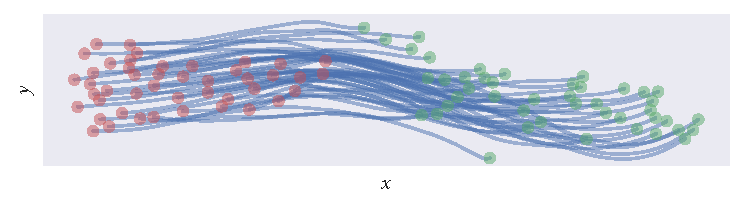
\includegraphics{seq_1_traj.pdf}
  \caption{The trajectories of sheep reconstructed from video footage of
    sequence $1$. The realised flock shows $45$ individuals moving cohesively
    over $192$ frames. The observations in the first frame of this sequence were
    used to seed the forward simulations in \cref{cha:sim_studies}.}
  \label{fig:seq_1_traj}
\end{figure}
\begin{figure}[tbp]
  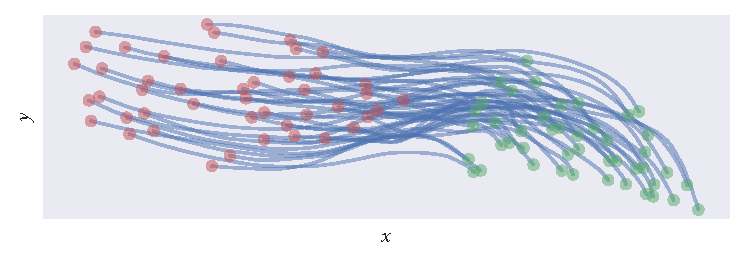
\includegraphics{seq_2_traj.pdf}
  \caption{A trajectory plot of the flock realised in sequence $2$. These
    trajectories correspond to those shown in the drone footage of
  \cref{fig:sheep_frame}.}
  \label{fig:seq_2_traj}
\end{figure}
\begin{figure}[tbp]
  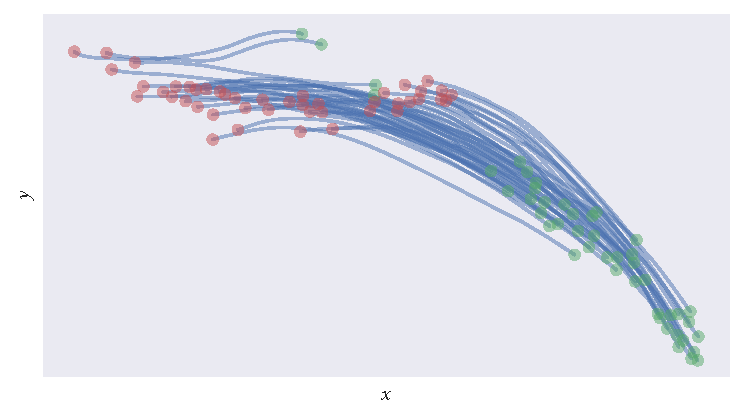
\includegraphics{seq_3_traj.pdf}
  \caption{Illustrating the movement of the flock in sequence $3$. Although
    this flock appears as cohesive as the events in sequences $1$ and $2$,
    this flock is also seen to go through greater directional changes.}
  \label{fig:seq_3_traj}
\end{figure}

The data realised by the drone captured footage resembles the data used in the
simulation studies of \cref{cha:sim_studies}. In fact, the first observed frame
of sequence $1$ was used to seed these forward simulations.
    
\section{Model fitting}

We now proceed to fit the global agent-based models introduced in
\cref{cha:model_dev} to the three flocking events realised. The performance of
these fitted models is then assessed by the Akaike Information Criteria. Model
adequacy is inspected with standardised residual plots and posterior predictive
checking.

\subsection{Sequence 1}

Sequence $1$ represents the most cohesive flocking event of the captured
sequences. We shall use the inference schemes constructed in
\cref{cha:sim_studies} to fit our candidate models to this data. With the
models fitted, we can then assess the performance of the model fits, and rank
the candidate models by their predictive performance.

\subsubsection{Posterior beliefs}

Our posterior beliefs about the parameters of the candidate models fitted to
sequence $1$ are shown in \cref{fig:posteriors_seq1}. Our prior beliefs about
the parameters are overlain in red. For all the inferred parameters our prior
beliefs appear flat in comparison to our posterior beliefs. This shows that we
were able to learn a lot from the data, and that our prior beliefs did not have
a strong impact on our posterior realisations.

Stan's No-U-Turn-Sampler was used to draw samples from the posterior
distributions of the Null, power-law weighted, Gaussian weighted and
topological models. To perform the model fittings we initialised four
independent Markov chains at draws from our prior beliefs. Chains were
simulated for $10,000$ iterations, with the first $5,000$ iterations discarded
to allow convergence. The samples drawn by each independent chain are
represented by the different coloured histograms of \cref{fig:posteriors_seq1}.
The overlain histograms show that the chains all converged to the same common
distribution.

The parameters of the Vicsek model were inferred by implementing a random walk
Metropolis--Hastings sampler. This algorithm was simulated for $10^6$
iterations, with the first half of the chains discarded to allow a burn-in
period. Our posterior beliefs about the interaction radius $r$, shown in
\cref{subfig:posterior_seq1_vicsek}, show a very strong negative skew. As our
posterior density rapidly drops to zero as $r\rightarrow3.25$, we conclude  
that at $r\approx3.25$ an agent suddenly includes the influence of a neighbour
which the model finds incompatible. This behaviour is a product of the
discontinuity of Vicsek's weighting rule.

The interaction parameters inferred from sequence $1$ all represent weak
interactions. This finding is consistent with the observation that weak
alignment interactions are sufficient to maintain groups which are already
highly polarised \parencite{jhawar20}. The small values inferred for the
parameter $\nu$, representing the degrees of freedom of the Student's
$t$-distribution, suggests evidence of non-normality of the noise. This result
is significant as thus far the assumption of normally distributed noise has
been a mainstay of agent-based modelling.

Although we have shown that our candidate models \emph{can} be fit to sequence
$1$, this does not say anything about their adequacy or goodness-of-fit. To
assess goodness-of-fit we shall inspect residual plots and make posterior
predictive checks.

\begin{figure}[p]
  \captionsetup[subfigure]{aboveskip=0pt,
                           belowskip=6pt,
                           oneside,
                           margin={0.7cm,0cm}}
  \begin{subfigure}[b]{\textwidth}
    \centering
    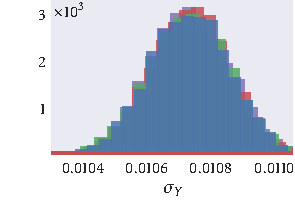
\includegraphics{seq1/null_hist_sigma_Y.pdf}%
    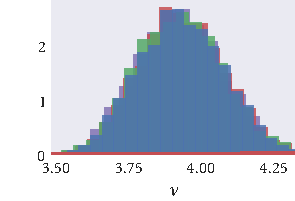
\includegraphics{seq1/null_hist_nu.pdf}
    \caption{Null model}
    \label{subfig:posterior_seq1_null}
  \end{subfigure}
  \begin{subfigure}[b]{\textwidth}
    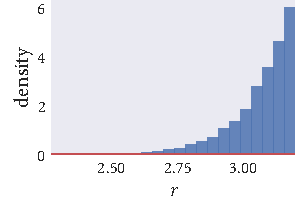
\includegraphics{seq1/r_hist_r.pdf}%
    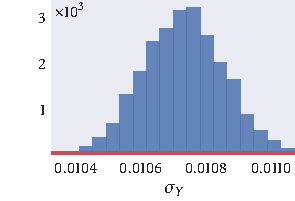
\includegraphics{seq1/r_hist_sigma_Y.pdf}%
    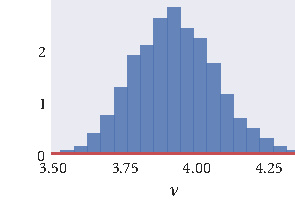
\includegraphics{seq1/r_hist_nu.pdf}
    \caption{Vicsek model}
    \label{subfig:posterior_seq1_vicsek}
  \end{subfigure}
  \begin{subfigure}[b]{\textwidth}
    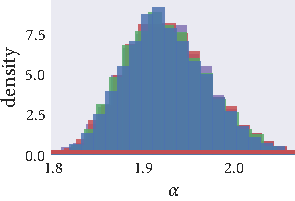
\includegraphics{seq1/power_hist_alpha.pdf}%
    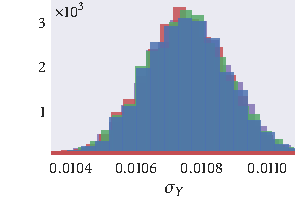
\includegraphics{seq1/power_hist_sigma_Y.pdf}%
    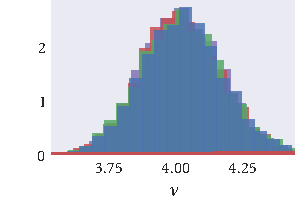
\includegraphics{seq1/power_hist_nu.pdf}
    \caption{Power-law weighted model}
    \label{subfig:posterior_seq1_power}
  \end{subfigure}
  \begin{subfigure}[b]{\textwidth}
    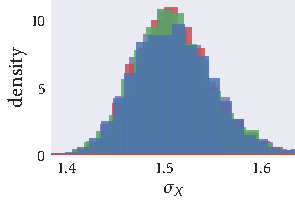
\includegraphics{seq1/gauss_hist_sigma_X.pdf}%
    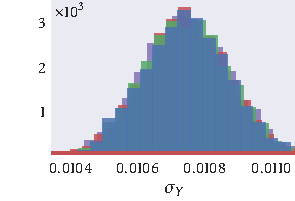
\includegraphics{seq1/gauss_hist_sigma_Y.pdf}%
    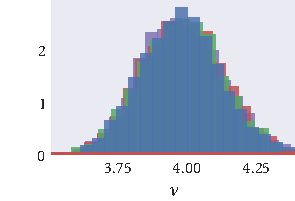
\includegraphics{seq1/gauss_hist_nu.pdf}
    \caption{Gaussian weighted model}
    \label{subfig:posterior_seq1_gauss}
  \end{subfigure}
  \begin{subfigure}[b]{\textwidth}
    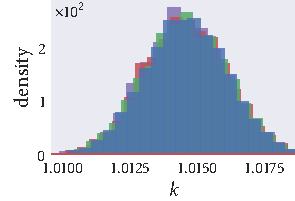
\includegraphics{seq1/top_hist_k.pdf}%
    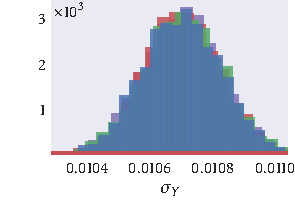
\includegraphics{seq1/top_hist_sigma_Y.pdf}%
    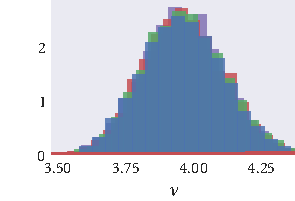
\includegraphics{seq1/top_hist_nu.pdf}%
    \caption{Topological model}
    \label{subfig:posterior_seq1_top}
  \end{subfigure}
  \vspace{-1.5em}
  \caption{Histogram plots show the posterior samples realised in fitting
    candidate models to the data of sequence $1$. Our priors beliefs are overlain
    in red, and in all cases appear flat in comparison to our posterior
    beliefs; this indicates that the observed data has been very informative.}
  \label{fig:posteriors_seq1}
\end{figure}

\subsubsection{Standardised residuals}

Assessing plots of residuals can be used as an informal method to assess
modelling assumptions. To compare model and residual, we first rearrange
\cref{eq:students_update} to see that:
\begin{equation*}
  (\theta_{i,t+1} - \angmean{\theta}_{i,t}) / \sigma_Y \given \nu \sim t_{\nu},
\end{equation*}
where $t_{\nu}$ is the standardised Student's $t$-distribution with $\nu$
degrees of freedom. To realise a model's residuals we compute
$\angmean{\theta}_{i,t}$ for $i=1,\ldots,N$ and $t=1,\ldots,T$ for every
posterior sample made by our inference scheme. The residuals can then be
computed as $\theta_{i,t+1} - \angmean{\theta}_{i,t}$ and standardised by
dividing by the posterior mean of the scale parameter $\sigma_Y$. The residuals
are compared with the model graphically by overlaying a standardised Student's
$t$-distribution with the degrees of freedom parameter taken from our posterior
mean.

\cref{fig:residuals_seq1} shows the standardised residuals of our fitted
models. We see that all the models look to give a good fit to the data. It may
come as a surprise that the Null model looks to perform so well. However, this
is again a product of the observation that our flock was already highly
polarised, and that only weak alignment interactions are necessary to maintain
a flock which is already cohesive.

\begin{figure}[tbb]
  \captionsetup[subfigure]{aboveskip=2pt,
                           belowskip=9pt,
                           oneside,
                           margin={0.7cm,0cm}}
  \begin{subfigure}[b]{0.33333\textwidth}
    \caption{Null model}
    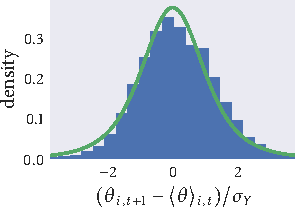
\includegraphics{seq1/null_residuals.pdf}
  \end{subfigure}\hspace{2pt}
  \begin{subfigure}[b]{0.33333\textwidth}
    \caption{Vicsek model}
    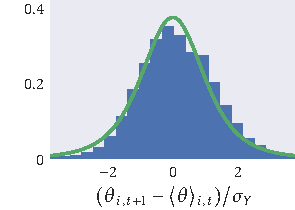
\includegraphics{seq1/r_residuals.pdf}
  \end{subfigure}\vspace{1em}\\
  \begin{subfigure}[b]{0.33333\textwidth}
    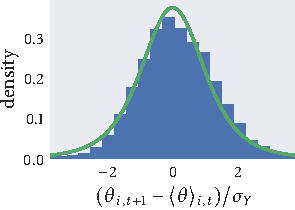
\includegraphics{seq1/power_residuals.pdf}
    \caption{Power-law weighted model}
  \end{subfigure}%
  \begin{subfigure}[b]{0.33333\textwidth}
    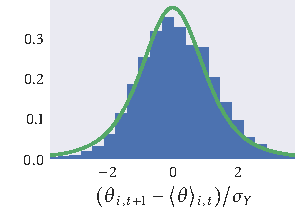
\includegraphics{seq1/gauss_residuals.pdf}
    \caption{Gaussian weighted model}
  \end{subfigure}%
  \begin{subfigure}[b]{0.33333\textwidth}
    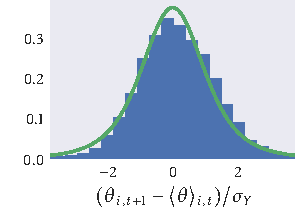
\includegraphics{seq1/top_residuals.pdf}
    \caption{Topological model}
  \end{subfigure}
  \caption{Standardised residuals of the models fitted to sequence $1$. The
  residuals are standardised by dividing by the posterior mean of the scale
  parameter $\sigma_Y$. A Student's $t$-distribution with $\nu$ degrees of
  freedom taken from our posterior mean is overlain in green. We see that
  models all look to provide a good fit to the data.}
  \label{fig:residuals_seq1}
\end{figure}

Although plots of standardised residuals provide a useful informal measure of
model fit, it can be useful to use more formal methods such as information
criteria to quantify fit.

\subsubsection{Model rankings}

Akaike Information Criteria (AIC) favours models which better explain the
given data, expressed through a larger likelihood, but penalises model
complexity---quantified as the number of model parameters. The Akaike weight of
a model can be computed from its AIC value. Typically a model's Akaike weight is
interpreted as the probability that the model will make the best predictions on
new data, conditional on the set of models considered.

In \cref{tab:aic_seq1} we show the value of AIC computed for each model fit.
Recall that \emph{smaller} values of AIC indicate a \emph{better} estimate of
predictive performance. \cref{tab:aic_seq1} shows the ranking of each model
fit. We see that the topological model was ranked as the best performing model,
followed by the power-law and Gaussian weighted models. The Null and Vicsek
models are ranked as the worst performing. If we were to only compare maximised
likelihoods we would rank the Null and Vicsek models the same. However, AIC
penalises for model complexity, and so having an extra model parameter without
being better at describing the data: the Vicsek model is ranked below the Null
model.

\begin{table}[tbp]
\begin{tabular}{@{}lrrrrr@{}}
\toprule
Model                       &      AIC & rank & pAIC & dAIC & weight \\
\midrule
Topological                 & -49\,031 &    1 &  3 &  0.0 &   0.98 \\
Power-law                   & -49\,023 &    2 &  3 &  7.4 &   0.02 \\
Gaussian                    & -48\,985 &    3 &  3 & 46.3 &   0.00 \\
Null                        & -48\,943 &    4 &  2 & 87.7 &   0.00 \\
Vicsek                      & -48\,941 &    5 &  3 & 89.7 &   0.00 \\
\bottomrule
\end{tabular}
\caption{Tabulated values of AIC and the corresponding Akaike weights
  (displayed to $2$ decimal places) of each model fitted to sequence $1$. Models
  are ranked from $1$--$5$, where $1$ is the best fit and $5$ is the worst.}
\label{tab:aic_seq1}
\end{table}

\subsubsection{Posterior predictive checks}

Forward simulating candidate models with parameters drawn from our posterior
beliefs provides an informal method to assess how well a model can reproduce
realistic behaviours. Here we forward simulate each candidate model one
thousand times. To initialise each simulation we randomly draw model parameters
from our posterior beliefs. We simulate the movement of $45$ sheep, initially
positioned and directed as in the first frame of the fitted sequence, for $192$
time steps. We compute the alignment of the flocks at each time step.

\cref{fig:checks_seq1} shows the alignment of the simulated flocks. The top
panel shows the alignment of two sets of randomly selected simulations. We see
that all the models do a reasonable job of capturing the observed flock
alignment for the first $\approx25$ time steps. After this, the observed flock
experiences a fluctuation in alignment over a time scale of $\approx100$
frames. Our models do not appear capable of producing flocks with such
long-range fluctuations in alignment. This may indicate the presence of
interactions or external influences not accounted for by our models. It may
also suggest the presence of a longer range dependence on previous directions.

\begin{figure}[tbp]
  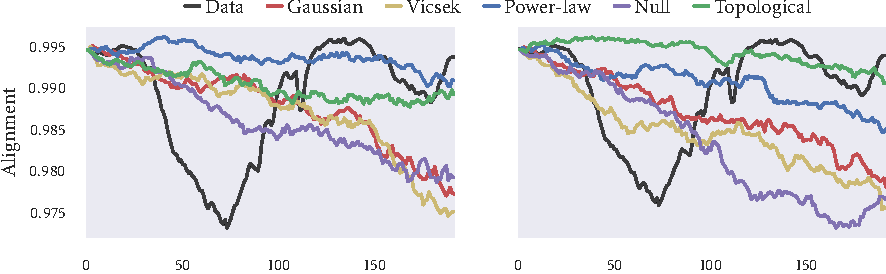
\includegraphics{alignment/alignment_single_1.pdf}\vspace{1em}\\
  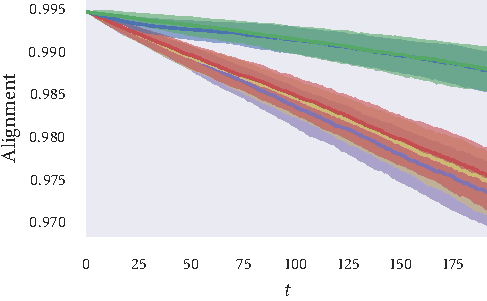
\includegraphics{alignment/alignment_ensemble_1.pdf}
  \caption{The alignment of flocks forward simulated with parameters drawn
    from our posterior beliefs. The top panels show two randomly selected sets
    of forward simulations. The bottom panel shows the median alignment across
    all simulations. Bands represent the upper and lower quartiles of
    the alignments computed at each time step.}
  \label{fig:checks_seq1}
\end{figure}

The bottom panel of \cref{fig:checks_seq1} shows the median alignment of
simulated flocks as a function of time. The coloured bands around the medians
show the upper and lower quartiles of the realised alignments. We see that the
topological and Gaussian models, favoured by AIC, produce the most consistently
cohesive flocks.

\subsection{Sequence 2}

This sequences details the movements of our flock of $45$ sheep over $183$
frames. The recorded flock is again very coherent and highly polarised.

\subsubsection{Posterior beliefs}

\begin{figure}[p]
  \captionsetup[subfigure]{aboveskip=1pt,
                           belowskip=9pt,
                           oneside,
                           margin={0.7cm,0cm}}
  \begin{subfigure}[b]{\textwidth}
    \centering
    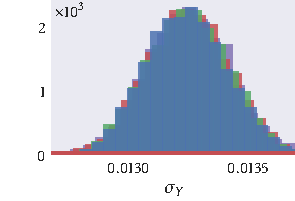
\includegraphics{seq2/null_hist_sigma_Y.pdf}\hspace{0.01\textwidth}
    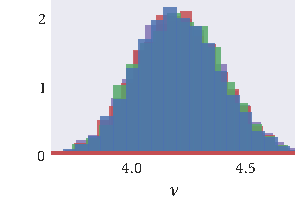
\includegraphics{seq2/null_hist_nu.pdf}
    \caption{Null model}
  \end{subfigure}
  \begin{subfigure}[b]{\textwidth}
    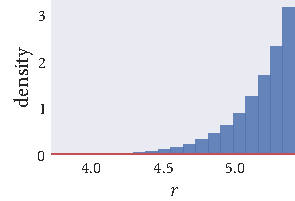
\includegraphics{seq2/r_hist_r.pdf}%
    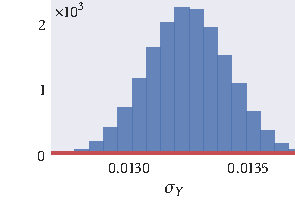
\includegraphics{seq2/r_hist_sigma_Y.pdf}%
    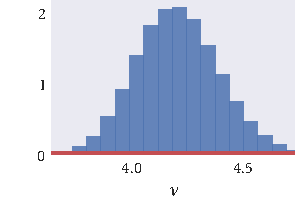
\includegraphics{seq2/r_hist_nu.pdf}
    \caption{Vicsek model}
  \end{subfigure}
  \begin{subfigure}[b]{\textwidth}
    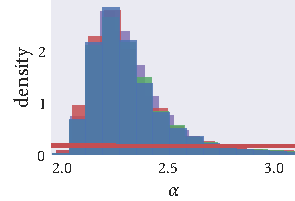
\includegraphics{seq2/power_hist_alpha.pdf}%
    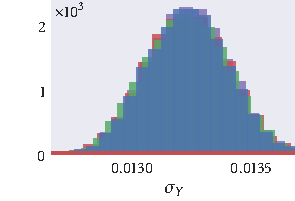
\includegraphics{seq2/power_hist_sigma_Y.pdf}%
    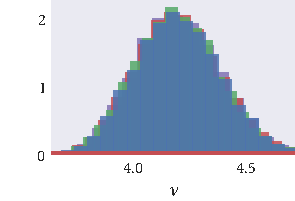
\includegraphics{seq2/power_hist_nu.pdf}
    \caption{Power-law weighted model}
  \end{subfigure}
  \begin{subfigure}[b]{\textwidth}
    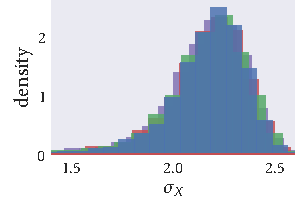
\includegraphics{seq2/gauss_hist_sigma_X.pdf}%
    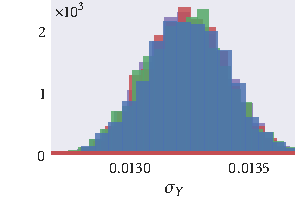
\includegraphics{seq2/gauss_hist_sigma_Y.pdf}%
    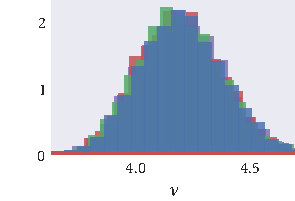
\includegraphics{seq2/gauss_hist_nu.pdf}
    \caption{Gaussian weighted model}
  \end{subfigure}
  \begin{subfigure}[b]{\textwidth}
    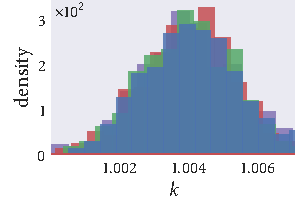
\includegraphics{seq2/top_hist_k.pdf}%
    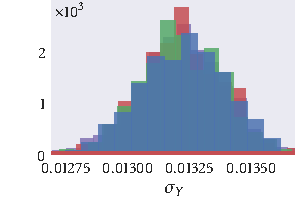
\includegraphics{seq2/top_hist_sigma_Y.pdf}%
    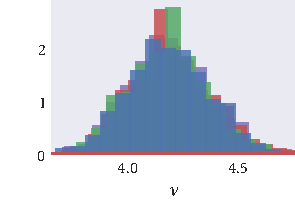
\includegraphics{seq2/top_hist_nu.pdf}%
    \caption{Topological model}
  \end{subfigure}
  \vspace{-1.75em}
  \caption{Posterior realisations of the model parameters inferred in fitting
  candidate models to sequence $2$. Posterior samples of the parameters of the
  Vicsek model were drawn by the implementation of a Metropolis--Hastings
  sampler. The remaining models were fitted with the implementation of Stan's
  NUTS algorithm.}
  \label{fig:posteriors_seq2}
\end{figure}

\subsubsection{Standardised residuals}

\begin{figure}[tbp]
  \captionsetup[subfigure]{aboveskip=2pt,
                           belowskip=9pt,
                           oneside,
                           margin={0.7cm,0cm}}
  \begin{subfigure}[b]{0.33333\textwidth}
    \caption{Null model}
    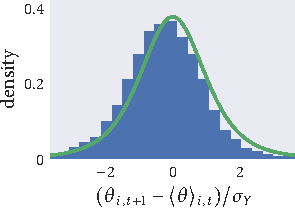
\includegraphics{seq2/null_residuals.pdf}
  \end{subfigure}\hspace{2pt}
  \begin{subfigure}[b]{0.33333\textwidth}
    \caption{Vicsek model}
    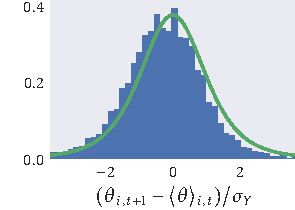
\includegraphics{seq2/r_residuals.pdf}
  \end{subfigure}\vspace{1em}\\
  \begin{subfigure}[b]{0.33333\textwidth}
    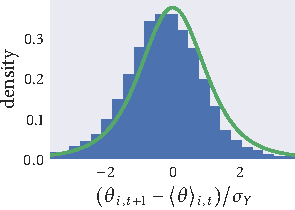
\includegraphics{seq2/power_residuals.pdf}
    \caption{Power-law weighted model}
  \end{subfigure}%
  \begin{subfigure}[b]{0.33333\textwidth}
    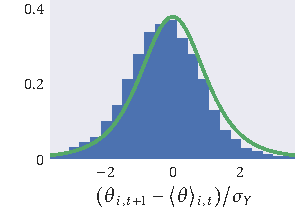
\includegraphics{seq2/gauss_residuals.pdf}
    \caption{Gaussian weighted model}
  \end{subfigure}%
  \begin{subfigure}[b]{0.33333\textwidth}
    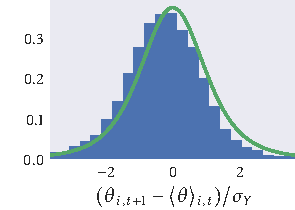
\includegraphics{seq2/top_residuals.pdf}
    \caption{Topological model}
  \end{subfigure}
  \caption{Standardised residuals of models fitted to sequence $2$.}
  \label{fig:residuals_seq2}
\end{figure}

\subsubsection{Model rankings}

\begin{table}[tbp]
\begin{tabular}{@{}lrrrrr@{}}
\toprule
Model                       &        AIC & rank & pAIC & dAIC & weight \\
\midrule
Power-law                   & -43\,495 &    1 &  3.0 &  0.0 &   0.49 \\
Topological                 & -43\,494 &    2 &  3.0 &  0.2 &   0.44 \\
Gaussian                    & -43\,490 &    3 &  3.0 &  4.5 &   0.05 \\
Null                        & -43\,488 &    4 &  2.0 &  6.9 &   0.02 \\
Vicsek                      & -43\,486 &    5 &  3.0 &  8.9 &   0.01 \\
\bottomrule
\end{tabular}
\caption{Fits to sequence $2$.}
\label{tab:aic_seq2}
\end{table}

\subsubsection{Posterior predictive checks}

\begin{figure}[tbp]
    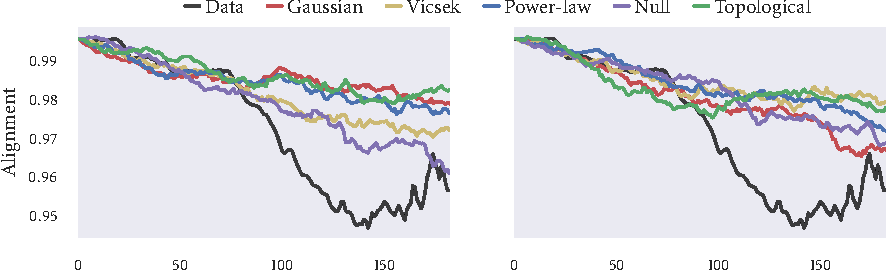
\includegraphics{alignment/alignment_single_2.pdf}\vspace{1em}\\
    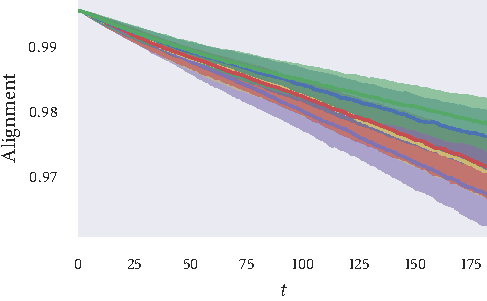
\includegraphics{alignment/alignment_ensemble_2.pdf}
    \caption{Posterior predictive checks for sequence $2$.}
    \label{fig:checks_seq2}
\end{figure}

\subsection{Sequence 3}

\subsubsection{Posterior beliefs}

\begin{figure}[p]
  \captionsetup[subfigure]{aboveskip=0pt,
                           belowskip=9pt,
                           oneside,
                           margin={0.7cm,0cm}}
  \begin{subfigure}[b]{\textwidth}
    \centering
    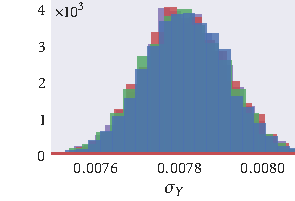
\includegraphics{seq3/null_hist_sigma_Y.pdf}\hspace{0.01\textwidth}
    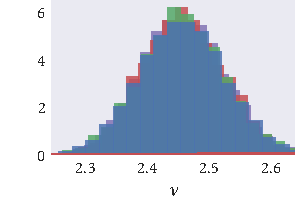
\includegraphics{seq3/null_hist_nu.pdf}
    \caption{Null model}
  \end{subfigure}
  \begin{subfigure}[b]{\textwidth}
    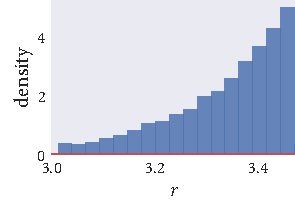
\includegraphics{seq3/r_hist_r.pdf}%
    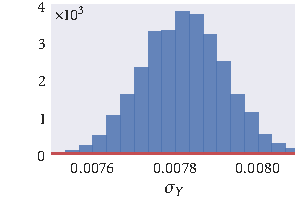
\includegraphics{seq3/r_hist_sigma_Y.pdf}%
    \includegraphics{seq3/r_hist_nu.pdf}
    \caption{Vicsek model}
  \end{subfigure}
  \begin{subfigure}[b]{\textwidth}
    \includegraphics{seq3/power_hist_alpha.pdf}%
    \includegraphics{seq3/power_hist_sigma_Y.pdf}%
    \includegraphics{seq3/power_hist_nu.pdf}
    \caption{Power-law weighted model}
  \end{subfigure}
  \begin{subfigure}[b]{\textwidth}
    \includegraphics{seq3/gauss_hist_sigma_X.pdf}%
    \includegraphics{seq3/gauss_hist_sigma_Y.pdf}%
    \includegraphics{seq3/gauss_hist_nu.pdf}
    \caption{Gaussian weighted model}
  \end{subfigure}
  \begin{subfigure}[b]{\textwidth}
    \includegraphics{seq3/top_hist_k.pdf}%
    \includegraphics{seq3/top_hist_sigma_Y.pdf}%
    \includegraphics{seq3/top_hist_nu.pdf}%
    \caption{Topological model}
  \end{subfigure}
  \caption{Posterior beliefs of model fits to sequence $3$.}
  \label{fig:posteriors_seq3}
\end{figure}

\subsubsection{Standardised residuals}

\begin{figure}[tbp]
  \captionsetup[subfigure]{aboveskip=2pt,
                           belowskip=9pt,
                           oneside,
                           margin={0.7cm,0cm}}
  \begin{subfigure}[b]{0.33333\textwidth}
    \caption{Null model}
    \includegraphics{seq3/null_residuals.pdf}
  \end{subfigure}\hspace{2pt}
  \begin{subfigure}[b]{0.33333\textwidth}
    \caption{Vicsek model}
    \includegraphics{seq3/r_residuals.pdf}
  \end{subfigure}\vspace{1em}\\
  \begin{subfigure}[b]{0.33333\textwidth}
    \includegraphics{seq3/power_residuals.pdf}
    \caption{Power-law weighted model}
  \end{subfigure}%
  \begin{subfigure}[b]{0.33333\textwidth}
    \includegraphics{seq3/gauss_residuals.pdf}
    \caption{Gaussian weighted model}
  \end{subfigure}%
  \begin{subfigure}[b]{0.33333\textwidth}
    \includegraphics{seq3/top_residuals.pdf}
    \caption{Topological model}
  \end{subfigure}
  \caption{Standardised residuals of models fitted to sequence $3$.}
  \label{fig:residuals_seq3}
\end{figure}

\subsubsection{Model rankings}

\begin{table}[tbp]
\begin{tabular}{@{}lrrrrr@{}}
\toprule
Model                       &        AIC & rank & pAIC &  dAIC & weight \\
\midrule
Power-law                   & -52\,242 &    1 &  3.0 &   0.0 &   1.00 \\
Gaussian                    & -52\,222 &    2 &  3.0 &  20.3 &   0.00 \\
Topological                 & -52\,169 &    3 &  3.0 &  73.6 &   0.00 \\
Null                        & -52\,037 &    4 &  2.0 & 205.8 &   0.00 \\
Vicsek                      & -52\,026 &    6 &  3.0 & 216.1 &   0.00 \\
\bottomrule
\end{tabular}
\caption{Fits to sequence $3$.}
\label{tab:aic_seq3}
\end{table}

\subsubsection{Posterior predictive checks}

\begin{figure}[tbp]
    \includegraphics{alignment/alignment_single_3.pdf}\vspace{1em}\\
    \includegraphics{alignment/alignment_ensemble_3.pdf}
    \caption{Posterior predictive checks for sequence $3$.}
    \label{fig:checks_seq3}
\end{figure}


